%!TEX root=../main.tex
% Chapter Template

\chapter{Experimental Validation} % Main chapter title

\label{Validation} % Change X to a consecutive number; for referencing this chapter elsewhere, use \ref{ChapterX}

%----------------------------------------------------------------------------------------
%	SECTION 1
%----------------------------------------------------------------------------------------

This section takes a look at the validation of the system from different viewpoints. A validation of the code is described in terms of integration tests. The recommendations are validated statistically by using two standard measures. Concrete examples of recommendations are given to provide some insight into what kind of recommendations are provided for different visitors.

\section{Integration tests}
The code is validated through a series of top-down, black-box integration tests. The purpose of these tests is to ensure the functionality of the two controllers, \textit{ProductRecommendationController} and \textit{DataController}. An overview of the test cases can be seen in table \ref{testCases}.

\begin{table}[H]
\centering
\caption{Integration test cases}
\label{testCases}
\begin{tabular}{|p{6cm}|p{5cm}|p{5cm}|}
\hline
\textbf{Method}             & \textbf{Test Case}                                             & \textbf{Expected Result}           \\ \hline
GetRecommendationForVisitor & Valid arguments                                                & String array of size 5             \\ \hline
GetRecommendationForVisitor & Non existing visitor                                           & String array of size 5             \\ \hline
GetRecommendationForVisitor & Uppercase/lowercase visitorUID                                 & String array of size 5             \\ \hline
GetRecommendationForVisitor & Uppercase/lowercase database                                   & String array of size 5             \\ \hline
GetRecommendationForVisitor & Number of recommendations being larger than available products & String array of all valid products \\ \hline
GetRecommendationForVisitor & Visitor with no behavior                                       & String array of size 5             \\ \hline
GetRecommendationForVisitor & Non existing database                                          & Empty string array                 \\ \hline
PutVisitor                  & New visitor                                                    & HTTP status code 201 created         \\ \hline
PutVisitor                  & Existing visitor                                               & HTTP status code 400 Bad Request            \\ \hline
PutVisitor                  & Non existing database                                          & HTTP status code 400 Bad Request            \\ \hline
PutProduct                  & New product                                                    & HTTP status code 201 created         \\ \hline
PutProduct                  & Existing product                                               & HTTP status code 400 Bad Request            \\ \hline
PutProduct                  & Non existing database                                          & HTTP status code 400 Bad Request           \\ \hline
PutBehavior                 & New behavior                                                   & HTTP status code 200 OK         \\ \hline
PutBehavior                 & Non existing database                                          & HTTP status code 400 Bad Request          \\ \hline
\end{tabular}
\end{table}

Most of the tests of the recommendation part is tested with 5 recommendations being requested, hence the return of a string array with size 5. \\
The put methods should return \textit{HTTP status code 201 Created} if a new item is created in the database, \textit{200 OK} if an item is updated, and \textit{400 Bad Request} if it fails.
All tests run successfully and a result overview can be seen in figure \ref{testResult}
\begin{figure}[H]
\centering
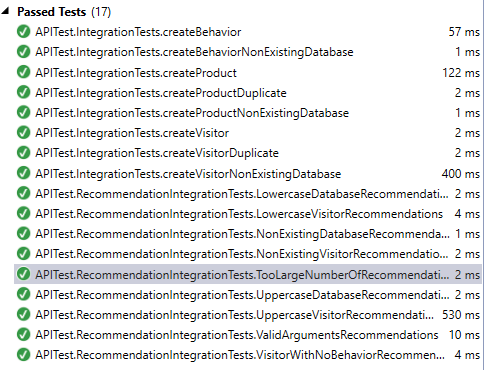
\includegraphics[scale=0.8]{testResults}
\caption{Result of all integration tests}
\label{testResult}
\end{figure}


\section{Validation of recommendations}

Validation of product recommendation engines is focused around two approaches \cite{eval}:
\begin{itemize}
	\item Offline validation
	\item Online validation
\end{itemize}


\subsection{Offline validation}
This section takes two approaches to validating the implemented recommendation engine:
\begin{itemize}
	\item A statistical approach using recall and precision
	\item Concrete examples
\end{itemize}

\subsubsection{Statistical approach}
Recall and Precision are two measures used for offline validation of product recommendation systems. Recall is defined as the number of relevant items (successful guesses) retrieved divided by the total number of relevant items (all behavior). Precision is defined as the number of relevant items retrieved divided by the total number of documents retrieved (all recommendations). \\ In recommendation systems the two measures are also described as follows: 
\begin{description}
	\item [Recall] \textit{a perfect recall score of 1.0 means that all good recommended items were suggested in the list (although says nothing about how many bad recommendations were also in the list)} \cite{recallAndPrecision}
	\item [Precision] \textit{a perfect precision score of 1.0 means that every item recommended in the list was good (although says nothing about if all good recommendations were suggested)} \cite{recallAndPrecision}
\end{description}

These measures are found using a method where a percentage of the data available is used as regular input data and another percentage as test data \cite{eval}. The evaluation run in this project used 80 percent of the data as input and tested on the remaining 20 percent. More specifically the remaining 20 percent was used in the following way:
\begin{itemize}
\item Take each visitor with more than two behaviors
\item Input half of the visitor's behaviors via the \gls{API}
\item Generate 5 recommendations for the specific visitor
\item See if the remaining half of his behaviors are in the recommended 5 items.
\end{itemize}
The selected 20\% visitors are chosen randomly as they are sorted by Id which is a randomized string assigned to each visitor.

This resulted in a total of 1,934 visitors tested and a total of 9670 recommendations. These visitors have 11,328 behaviors where half was used as input and half was used as control. This means the recommendation engine had to predict half of 11,328 (5,664) behaviors. The algorithm succeeded in correctly predicting 2974 behaviors.  \\
The recall percentage is calculated as \begin{math}2974/5664*100=52.5\%\end{math}. \\ The precision percentage is calculated as \begin{math}2974/9670*100=30.8\%\end{math}. \\
The Recall and Precision rates are visualized in figure \ref{recallAccuracy}. The result of this evaluation as well as the scripts used can be found attached with the source code. \\
\begin{figure}[H]
\centering
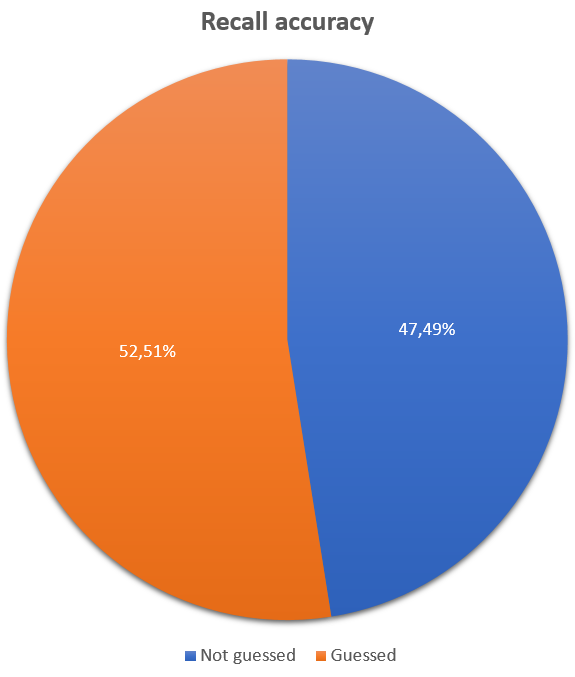
\includegraphics[scale=0.7]{recallAccuracy}
\caption{Recall accuracy}
\label{recallAccuracy}
\end{figure}
The engine only had half of each visitors behavior as input which could be as low as 1 behavior and still managed to guess correctly more than half of the time.
The precision score is only 30.8\% in this test which implies that the algorithm also provides many poor recommendations. One of the major drawbacks of these statistics is the fact that it assumes that every recommended item not in the visitors real behavior is a bad recommendation. This is not always the case as a visitor might not have looked at the product because he was unaware of its existence but might have decided to look at it if it was recommended \cite{evaluatingRecommender}. Another drawback is that the numbers tell nothing about catalog coverage which is how much of the product catalog the recommendation system recommends. It is therefore possible to have a good recall rate but not be suggesting anything new to the visitors \cite{eval}.
As the algorithm acquires more data on all visitors the precision should increase.\\
Root-Mean-Square-Error (RMSE) and Mean-Absolute-Error (MAE) \cite{rmseAndmae} are other measures used in offline validation. These measures require user ratings on products which is not present in the data for this project. RMSE and MAE can therefore not be used to evaluate these product recommendations. \\
\subsubsection{Concrete examples}
To give a better understanding of the recommendations given by the algorithm a few specific examples are given below. \\

\textbf{Visitor A} has looked at the following products:
\begin{itemize}
\item \textbf{36991: }Playset Brandmand Sam fyrtårn med figur
\item \textbf{37691: }Playset Brandmand Sam Havnestation
\item \textbf{37799: }Firman Sam Ocean Rescue
\item \textbf{38950: }Sejt Brandmand Sam udstyrssæt
\item \textbf{40786: }Brandmand Sam helikopter med lys og lyd
\item \textbf{42373: }Biler Brandmand Sam og brandbil
\item \textbf{52818: }Udklædning tilbehør sej Brandmand Sam megafon
\item \textbf{52919: }Playset Fireman Sam
\end{itemize}
and is recommended the following products:
\begin{itemize}
\item \textbf{43215: }Biler Brandmand Sam bil
\item \textbf{36991: }Payset Brandmand Sam fyrtårn med figur
\item \textbf{37799: }Firman Sam Ocean Rescue
\item \textbf{38950: }Sejt Brandmand Sam udstyrssæt med bælte
\item \textbf{34392:} Brandmand Sam 104 cm Fastelavnstøj
\end{itemize}

The visitor has already looked at some of the recommended items. As the recommendations size increases more new products to the visitor will appear. The recommendations are all "Brandmand Sam" products which is all he has looked at in the past. Whether it is good or bad depends on the business and how the visitors will respond. These recommendations are in accordance with the wishes of \gls{Struct} as they want very similar items to be recommended. Presenting the same products to a user several times can also increase the likelihood of a purchase happening. In the future the recommendation engine will be able to filter already purchased products, but this has yet to be implemented. \\\\

Another \textbf{visitor B} has looked at the following products:
\begin{itemize}
\item \textbf{43106: }Biler Scalextric C3528 BMW MINI Cooper S
\item \textbf{49777: }Scalextric Racerbane C1368 Bilbaner Le Mans Prototypes Sports Cars
\item \textbf{33136: }Chevrolet Camaro GT-R Biler Scalextric C3383 
\item \textbf{43104: }Scalextric C3524 VW Polo WRC Biler
\end{itemize}
and is recommended the following 5 products:
\begin{itemize}
\item \textbf{43106: }Biler Scalextric C3528 BMW MINI Cooper S
\item \textbf{43104: }Scalextric C3524 VW Polo WRC Biler
\item \textbf{49777: }Scalextric Racerbane C1368 Bilbaner Le Mans Prototypes Sports Cars
\item \textbf{33136: }Chevrolet Camaro GT-R Biler Scalextric C3383
\item \textbf{42841: }Maserati Trofeo Biler Scalextric C3388
\end{itemize}

These recommendations also relate closely to the products the visitor has viewed. \\\\

A final example \textbf{visitor C} has looked at these products:
\begin{itemize}
\item \textbf{42809: }Bosch arbejdsbord Bosch Værktøj og Værktøjsbænke
\item \textbf{42106: }Elsker du også bare paw patrol
\end{itemize}
and is recommended these products:
\begin{itemize}
\item \textbf{42106: }Elsker du også bare paw patrol
\item \textbf{42809: }Bosch arbejdsbord Bosch Værktøj og Værktøjsbænke
\item \textbf{40542: }LEGO Legends Of Chima Flyv op gennem skyerne
\item \textbf{31548:} LEGO Legends Of Chima Snurrende slyngplanter
\item \textbf{43713:} Fastelavnstøj Tid til at ringe efter politiet og Paw Patrols hund nummer 1
\end{itemize}
The two LEGO recommendations in this example might not seem thematically accurate, however since they have been recommended they must have a high similarity score to one or both of the products the visitor has looked at. A closer look at the data shows the two LEGO products to have similarity scores of 24 and 15 respectively to product 42106. Since these products are not in the same product group and have zero matching descriptions the high similarity score is the amount of times they have been looked at together with this product. The main product, product 42106, have been looked at by 9 other visitors and these 9 visitors have looked at the first LEGO product 24 times and the second LEGO product 15 times.

\subsection{Online validation}
When the recommendation algorithm is put into production, several new and better ways of evaluating the system becomes available. As the visitors get recommendations their behavior is logged and it is possible to see how many of the recommendations are actually used and adjust the algorithm thereafter. Online validations have not been possible as part of the project scope. In an online scenario the recommendations could be examined by calculating click-through rates and conversion rate. Click-through rate is how many percent of the recommendations have resulted in the visitor viewing the product. Conversion rate is how many percent of the recommendations have resulted in a purchase. Furthermore the turnover of the web shop can be analyzed over a period of time to measure whether or not the recommendations are effective.
This adjustment can potentially be automated by using machine learning - this is covered in more detail in chapter \ref{FutureWork}.

 